\documentclass[uplatex,a4j]{jsreport}
\usepackage{thesis}

\begin{document}
\chapter{HTML5字句解析仕様}
\label{字句解析仕様}
\section{概要}
%トークン,変数の説明=========
\subsection*{token}
HTML5字句解析器はHTML5の文章をtokenという単位に分解する.
字句解析器により排出されたトークンはDOMツリーを構成する次のステップに使われる.
排出されるtokenには,5つ種類があり,
その文書で利用するHTMLやXHTMLのバージョンを表すDOCTYPE token, "$<$!-- --$>$"などでコメントアウトした文章を表すcomment token, $<$,$>$で囲まれているタグを表すstart tag tokenとend tag token, 
文字を表すcharacter token, 文章の終了を表すend-of-file tokenがある.\\

DOCTYPE tokenはDOCTYPEの名前,  public identifierとsystem identifierの値, force-quirks flagの要素を持っている.\\
start tag token, end tag tokenはタグの名前, タグの属性の集合(attributes), self-closing flagの要素を持っている.\\
end-of-fileトークンが排出されたら字句解析器の動作は終了する.\\
\subsection*{変数}
HTML5字句解析器はreturn stateや一時バッファなどの変数を持つ.
%=========
\subsection*{状態}
HTML5字句解析仕様はWHATWG communityのwebサイトから得られる.~\cite{html5specification}\\
HTML5の字句解析器は80個の状態のあるオートマトンとして定義されている.
それぞれの状態は以下の図\ref{html5}の形式で書かれている.\\
\begin{figure}[h]
    \centering
    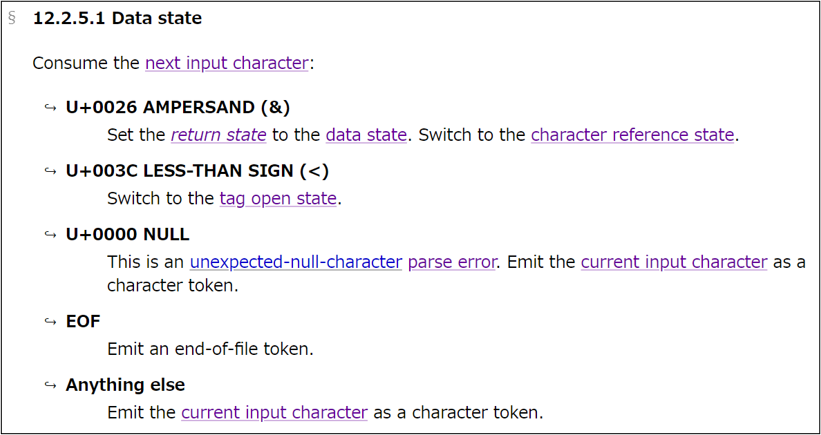
\includegraphics[keepaspectratio, scale=1.0]
         {figure/html5.png}
    \caption{HTML5字句解析仕様書}
    \label{html5}
\end{figure}

\section{動作の例}
\subsection{例1}
入力"$<$a$>$bc$<$/a$>$"に対して, HTML5字句解析器は以下のように動作を行う.\\
\begin{enumerate}
    \item 初期状態Data stateから, 文字'$<$'が消費され, Tag open state に遷移する.
    \item 文字'a'を消費し, 名前が空文字である新たなstart tag tokenを作る. Tag name stateに遷移する.
    \item 先ほど消費した文字'a'を再度消費し, start tag tokenの名前に'a'を付け足す.
    \item 文字'$>$'を消費し, start tag tokenを排出し, Data stateに遷移する.
    \item 文字'b'を消費し, characterToken('b')を排出する.
    \item 文字'c'を消費し, characterToken('c')を排出する.
    \item 文字'$<$'を消費し, Tag open state に遷移する.
    \item 文字'/'を消費し, End tag open state に遷移する.
    \item 文字'a'を消費し, 名前が空文字である新たなend tag tokenを作る. Tag name stateに遷移する.
    \item 先ほど消費した文字'a'を再度消費し, end tag tokenの名前に'a'を付け足す.
    \item 文字'$>$'を消費し, end tag tokenを排出し, Data stateに遷移する.
    \item end-of-file tokenを排出する.
\end{enumerate}
動作の結果として,\\
startTagToken(name = "a", attributes = []), characterToken('b'), characterToken('c'), endTagToken(name = "a"), end-of-fileToken\\
が順に排出される.

\subsection{例2}
%エラーが出る例
入力"a$<$ab"に対して, HTML5字句解析器は以下ように動作を行う.\\
\begin{enumerate}
    \item 初期状態Data stateにおいて, 文字'a'を消費し, characterToken('a')を排出する.
    \item 文字'$<$'を消費し, Tag open state に遷移する.
    \item 文字'a'を消費し, 名前が空文字である新たなstart tag tokenを作る. Tag name stateに遷移する.
    \item 先ほど消費した文字'a'を再度消費し, start tag tokenの名前に'a'を付け足す.
    \item 文字'b'を消費し, start tag tokenの名前に'b'を付け足す.
    \item "eof-in-tag"構文エラーを出す. end-of-file tokenを排出する.
\end{enumerate}
動作の結果として,\\
characterToken('a'), end-of-fileTokenが順に排出される.
\end{document}